\hypertarget{a00003}{
\section{eqOsg::Config Class Reference}
\label{a00003}\index{eqOsg::Config@{eqOsg::Config}}
}
This class handles the \hyperlink{a00045}{eqOsg} basic config for Equalizer.  


{\tt \#include $<$Config.h$>$}

Inherited by \hyperlink{a00004}{crf::crfConfig}.

Collaboration diagram for eqOsg::Config:\nopagebreak
\begin{figure}[H]
\begin{center}
\leavevmode
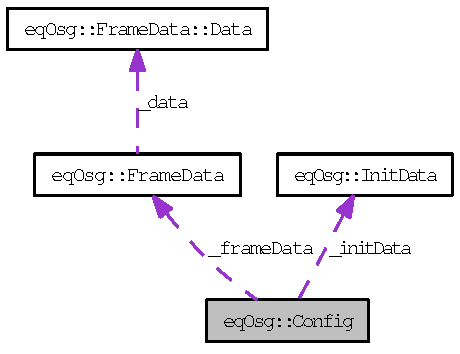
\includegraphics[width=257pt]{a00090}
\end{center}
\end{figure}
\subsection*{Public Member Functions}
\begin{CompactItemize}
\item 
\hyperlink{a00003_64865580c67831fd92e8c5222f0554cc}{Config} (eq::base::RefPtr$<$ eq::Server $>$ parent)
\begin{CompactList}\small\item\em Calls the base constructor and initialises the camera. \item\end{CompactList}\item 
virtual bool \hyperlink{a00003_73ab12bbf273fd4ff7e2dea65ee3e6f8}{init} ()
\begin{CompactList}\small\item\em Initialises our distributet data and calls the eq::Config::init(). \item\end{CompactList}\item 
virtual bool \hyperlink{a00003_e656952f262b9e5c3354583a04068b97}{exit} ()
\begin{CompactList}\small\item\em When exiting the configuration, the distributed data gets deregistered after the base eq::Config::exit() was called. \item\end{CompactList}\item 
virtual uint32\_\-t \hyperlink{a00003_955b3c5ffe177012da10434fbc8da7e0}{startFrame} ()
\begin{CompactList}\small\item\em Starts the new frame for rendering. \item\end{CompactList}\item 
virtual bool \hyperlink{a00003_0ac41bd28010ff7f7638beb051b6c9b9}{handleEvent} (const eq::ConfigEvent $\ast$event)
\begin{CompactList}\small\item\em Reimplemented for camera controls. \item\end{CompactList}\item 
virtual void \hyperlink{a00003_eac7f3b423d994667bac2007c5d78cc1}{setInitData} (const \hyperlink{a00011}{InitData} \&data)
\begin{CompactList}\small\item\em Reimplemented to register the framedata object. \item\end{CompactList}\item 
const \hyperlink{a00011}{InitData} \& \hyperlink{a00003_8a5b1862bf80067322a3a0b1f530f751}{getInitData} () const 
\begin{CompactList}\small\item\em Returns the initData. \item\end{CompactList}\item 
bool \hyperlink{a00003_140db32dd04daba4cb95233e180b0327}{mapData} (const uint32\_\-t initDataID)
\begin{CompactList}\small\item\em Maps our initData. \item\end{CompactList}\end{CompactItemize}
\subsection*{Protected Member Functions}
\begin{CompactItemize}
\item 
virtual void \hyperlink{a00003_b7754b48a74e7927643d3e2e6ca3c8ed}{updateCamera} (float elapsed)
\begin{CompactList}\small\item\em calculates the new properties for the camera \item\end{CompactList}\item 
\hypertarget{a00003_be9b795ee7263d5e8343fbd4c7a00ded}{
virtual void \hyperlink{a00003_be9b795ee7263d5e8343fbd4c7a00ded}{updateFrameData} ()}
\label{a00003_be9b795ee7263d5e8343fbd4c7a00ded}

\begin{CompactList}\small\item\em adds the new properties for framedata \item\end{CompactList}\item 
virtual bool \hyperlink{a00003_b66ac34d32b4e160ec19cb39231395ac}{handleCameraEvents} (const eq::ConfigEvent $\ast$event)
\begin{CompactList}\small\item\em If a keypress happens, this function updates \_\-moveDirection, so that the new camera position can be calculated in \hyperlink{a00003_b7754b48a74e7927643d3e2e6ca3c8ed}{updateCamera()}. \item\end{CompactList}\end{CompactItemize}
\subsection*{Protected Attributes}
\begin{CompactItemize}
\item 
\hypertarget{a00003_26a7379aa8c578f1bd7d404256b70932}{
\hyperlink{a00010}{FrameData} \hyperlink{a00003_26a7379aa8c578f1bd7d404256b70932}{\_\-frameData}}
\label{a00003_26a7379aa8c578f1bd7d404256b70932}

\begin{CompactList}\small\item\em The distributed frame data. \item\end{CompactList}\end{CompactItemize}


\subsection{Detailed Description}
This class handles the \hyperlink{a00045}{eqOsg} basic config for Equalizer. 

The Equalizer related event handling is done here. The \hyperlink{a00045}{eqOsg} basic camera calculations are done here as well. \begin{Desc}
\item[See also:]eq::Config \end{Desc}


\subsection{Constructor \& Destructor Documentation}
\hypertarget{a00003_64865580c67831fd92e8c5222f0554cc}{
\index{eqOsg::Config@{eqOsg::Config}!Config@{Config}}
\index{Config@{Config}!eqOsg::Config@{eqOsg::Config}}
\subsubsection[{Config}]{\setlength{\rightskip}{0pt plus 5cm}Config::Config (eq::base::RefPtr$<$ eq::Server $>$ {\em parent})}}
\label{a00003_64865580c67831fd92e8c5222f0554cc}


Calls the base constructor and initialises the camera. 

\begin{Desc}
\item[See also:]eq::Config::Config \end{Desc}


\subsection{Member Function Documentation}
\hypertarget{a00003_e656952f262b9e5c3354583a04068b97}{
\index{eqOsg::Config@{eqOsg::Config}!exit@{exit}}
\index{exit@{exit}!eqOsg::Config@{eqOsg::Config}}
\subsubsection[{exit}]{\setlength{\rightskip}{0pt plus 5cm}bool Config::exit ()\hspace{0.3cm}{\tt  \mbox{[}virtual\mbox{]}}}}
\label{a00003_e656952f262b9e5c3354583a04068b97}


When exiting the configuration, the distributed data gets deregistered after the base eq::Config::exit() was called. 

\begin{Desc}
\item[Returns:]True if everything worked fine. \end{Desc}
\hypertarget{a00003_8a5b1862bf80067322a3a0b1f530f751}{
\index{eqOsg::Config@{eqOsg::Config}!getInitData@{getInitData}}
\index{getInitData@{getInitData}!eqOsg::Config@{eqOsg::Config}}
\subsubsection[{getInitData}]{\setlength{\rightskip}{0pt plus 5cm}const {\bf InitData} \& Config::getInitData () const}}
\label{a00003_8a5b1862bf80067322a3a0b1f530f751}


Returns the initData. 

\begin{Desc}
\item[Returns:]The initData object. \end{Desc}
\hypertarget{a00003_b66ac34d32b4e160ec19cb39231395ac}{
\index{eqOsg::Config@{eqOsg::Config}!handleCameraEvents@{handleCameraEvents}}
\index{handleCameraEvents@{handleCameraEvents}!eqOsg::Config@{eqOsg::Config}}
\subsubsection[{handleCameraEvents}]{\setlength{\rightskip}{0pt plus 5cm}bool Config::handleCameraEvents (const eq::ConfigEvent $\ast$ {\em event})\hspace{0.3cm}{\tt  \mbox{[}protected, virtual\mbox{]}}}}
\label{a00003_b66ac34d32b4e160ec19cb39231395ac}


If a keypress happens, this function updates \_\-moveDirection, so that the new camera position can be calculated in \hyperlink{a00003_b7754b48a74e7927643d3e2e6ca3c8ed}{updateCamera()}. 

If a mouse move event happens, this function updates \_\-pointerXDiff and \_\-pointerYDiff, so that the new camera viewing direction can be calculated in \hyperlink{a00003_b7754b48a74e7927643d3e2e6ca3c8ed}{updateCamera()}. \begin{Desc}
\item[Parameters:]
\begin{description}
\item[{\em event}]The Equalizer event. \end{description}
\end{Desc}
\begin{Desc}
\item[Returns:]True if the event has been handled. \end{Desc}
\hypertarget{a00003_0ac41bd28010ff7f7638beb051b6c9b9}{
\index{eqOsg::Config@{eqOsg::Config}!handleEvent@{handleEvent}}
\index{handleEvent@{handleEvent}!eqOsg::Config@{eqOsg::Config}}
\subsubsection[{handleEvent}]{\setlength{\rightskip}{0pt plus 5cm}bool Config::handleEvent (const eq::ConfigEvent $\ast$ {\em event})\hspace{0.3cm}{\tt  \mbox{[}virtual\mbox{]}}}}
\label{a00003_0ac41bd28010ff7f7638beb051b6c9b9}


Reimplemented for camera controls. 

Handles the Equalizer events. If camera is enabled handleCameraEvents gets called \begin{Desc}
\item[Parameters:]
\begin{description}
\item[{\em event}]The event passed by Equalizer. \end{description}
\end{Desc}
\begin{Desc}
\item[Returns:]True, if the event has been handled \end{Desc}


toggle the eq cam switch

Update the cameras proberties by handling these events 

Reimplemented in \hyperlink{a00004_63938a0cf75d236b677c4cb147933b3c}{crf::crfConfig}.\hypertarget{a00003_73ab12bbf273fd4ff7e2dea65ee3e6f8}{
\index{eqOsg::Config@{eqOsg::Config}!init@{init}}
\index{init@{init}!eqOsg::Config@{eqOsg::Config}}
\subsubsection[{init}]{\setlength{\rightskip}{0pt plus 5cm}bool Config::init ()\hspace{0.3cm}{\tt  \mbox{[}virtual\mbox{]}}}}
\label{a00003_73ab12bbf273fd4ff7e2dea65ee3e6f8}


Initialises our distributet data and calls the eq::Config::init(). 

\begin{Desc}
\item[Returns:]True if everything succeed. \end{Desc}
\hypertarget{a00003_140db32dd04daba4cb95233e180b0327}{
\index{eqOsg::Config@{eqOsg::Config}!mapData@{mapData}}
\index{mapData@{mapData}!eqOsg::Config@{eqOsg::Config}}
\subsubsection[{mapData}]{\setlength{\rightskip}{0pt plus 5cm}bool Config::mapData (const uint32\_\-t {\em initDataID})}}
\label{a00003_140db32dd04daba4cb95233e180b0327}


Maps our initData. 

\begin{Desc}
\item[Parameters:]
\begin{description}
\item[{\em initDataID}]The initData's ID. \end{description}
\end{Desc}
\begin{Desc}
\item[Returns:]True if everything worked fine. \end{Desc}
\hypertarget{a00003_eac7f3b423d994667bac2007c5d78cc1}{
\index{eqOsg::Config@{eqOsg::Config}!setInitData@{setInitData}}
\index{setInitData@{setInitData}!eqOsg::Config@{eqOsg::Config}}
\subsubsection[{setInitData}]{\setlength{\rightskip}{0pt plus 5cm}void Config::setInitData (const {\bf InitData} \& {\em data})\hspace{0.3cm}{\tt  \mbox{[}virtual\mbox{]}}}}
\label{a00003_eac7f3b423d994667bac2007c5d78cc1}


Reimplemented to register the framedata object. 

\begin{Desc}
\item[Parameters:]
\begin{description}
\item[{\em data}]The init data object. \end{description}
\end{Desc}
\hypertarget{a00003_955b3c5ffe177012da10434fbc8da7e0}{
\index{eqOsg::Config@{eqOsg::Config}!startFrame@{startFrame}}
\index{startFrame@{startFrame}!eqOsg::Config@{eqOsg::Config}}
\subsubsection[{startFrame}]{\setlength{\rightskip}{0pt plus 5cm}uint32\_\-t Config::startFrame ()\hspace{0.3cm}{\tt  \mbox{[}virtual\mbox{]}}}}
\label{a00003_955b3c5ffe177012da10434fbc8da7e0}


Starts the new frame for rendering. 

Camera gets updated with the elapsed time, the frameData gets commited and the base startFrame function gets called. \begin{Desc}
\item[Returns:]Returns the frames ID \end{Desc}
\hypertarget{a00003_b7754b48a74e7927643d3e2e6ca3c8ed}{
\index{eqOsg::Config@{eqOsg::Config}!updateCamera@{updateCamera}}
\index{updateCamera@{updateCamera}!eqOsg::Config@{eqOsg::Config}}
\subsubsection[{updateCamera}]{\setlength{\rightskip}{0pt plus 5cm}void Config::updateCamera (float {\em elapsed})\hspace{0.3cm}{\tt  \mbox{[}protected, virtual\mbox{]}}}}
\label{a00003_b7754b48a74e7927643d3e2e6ca3c8ed}


calculates the new properties for the camera 

\begin{Desc}
\item[Parameters:]
\begin{description}
\item[{\em elapsed}]The elapsed time of th clock to create frame independent movement. \end{description}
\end{Desc}


The documentation for this class was generated from the following files:\begin{CompactItemize}
\item 
E:/schule/Thesis/Repo/trunk/crf/src/Config.h\item 
E:/schule/Thesis/Repo/trunk/crf/src/Config.cpp\end{CompactItemize}
